\documentclass[a4paper,12pt]{report}
\usepackage[utf8]{inputenc}
\usepackage[francais]{babel}
\usepackage{graphicx}
\usepackage{fancyhdr}
\usepackage[absolute]{textpos}
\usepackage[svgnames]{xcolor}
\usepackage{colortbl}
\usepackage{lastpage}
\usepackage{url}
\usepackage[hidelinks]{hyperref}
\usepackage{geometry}
\usepackage{tikz}
\usepackage{titlesec}
\usepackage{datetime}
\usepackage{lipsum}
\usepackage{supertabular}
\usetikzlibrary{matrix}

\newcommand{\doctitle}{VISION}
\newcommand{\doclongtitle}{Vision}

\title{\doctitle{} Vigilitate}
\author{Soules Kévin, Mercier Daniel, Budowski Prune, Harscoat Morgane, Poncet Manuel, Keller Flavien}
\date{\today}


\definecolor{myBlue}{RGB}{23,54,93}
\definecolor{lightGray}{gray}{0.7}
\newdateformat{slashdate}{\twodigit{\THEDAY}/\twodigit{\THEMONTH}/\THEYEAR}
\newcolumntype{R}[1]{>{\centering\let\newline\\\arraybackslash\hspace{0pt}}m{#1}}

\titleformat{\section}[block]{\bfseries}{\thesection.}{1em}{}
\titleformat{\subsection}[block]{\hspace{2em}}{\thesubsection}{1em}{}
\titleformat{\subsubsection}[block]{\hspace{3em}}{\thesubsubsection}{1em}{}
  
\geometry{
  a4paper,
  left=20mm,
  right=20mm,
}

\setlength{\unitlength}{1mm}
\addtolength{\headheight}{1.5\baselineskip}
\renewcommand{\headrulewidth}{0.0pt}
\renewcommand{\footrulewidth}{0.4pt}


\fancypagestyle{eip}{
  \fancyhf{}
  \fancyhead[L] {
    \includegraphics[width=3cm]{../../logos/logo_eip.png}
  }
  \fancyhead[R] {
    \colorbox{myBlue}{
      \textcolor{white}{
        \Large \textbf{[2017][Vigilate][\doctitle{}]}
      }
    }
  }
  \renewcommand{\headrulewidth}{0pt}
  \fancyfoot[L]{
    \textcolor{gray}{
      \{EPITECH.\}
    }
  }
  \fancyfoot[C]{Vigilate}
  \fancyfoot[R]{
    \ifnum\value{page}>0
    \thepage/\pageref{LastPage}
    \fi
  }
}

\makeatletter
\let\ps@plain\ps@eip
\makeatother

\pagestyle{eip}


\begin{document}
\date{\slashdate\today}
\setcounter{page}{-3}

% --- (1) Page de garde ---

\thispagestyle{empty}
\vspace*{\stretch{2}}
\begin{center}
  \textcolor{myBlue}{\Huge \textbf{EIP Vigilitate}}\linebreak
  \vspace*{\stretch{1}}
  \textcolor{gray}{\textit{\Large \doclongtitle{} (\doctitle{})}}\linebreak
  \vspace*{\stretch{1}}
  {\today}
\end{center}
\vspace*{\stretch{1}}
\newpage

% --- (2) Résumé ---

\vspace*{\stretch{1}}
\begin{flushleft}
  \textcolor{myBlue}{\textit{\large \textbf{Résumé du document}}}\linebreak
\end{flushleft}
Le cahier des charges commence par un bref rappel de notre EIP, Vigilate, un outil de sécurité informatique qui permet de se tenir informé des dernières vulnérabilités publiques rapidement sur tous les programmes que l’utilisateur souhaite vérifier. On mettra en avant les contraintes fonctionnelles et les exigences non-fonctionnelles comme le fait que notre projet doit être sécurisé, ou alors la réactivité de notre outil. Notre projet est réalisé par 6 personnes. Le document présente d’une part la structure du projet : un site web, le back-end, une machine virtuelle et un scanneur de programme et d’autre part, les différentes fonctionnalités du projet à partir d’un document UML (connexion de l’utilisateur, possibilité de modifier ses préférences : programmes à surveiller, style d’alerte souhaité...). Nous présentons dans la partie 6 l’organisation prévue : 2 personnes sur le site web, 2 sur le back-end, 1 sur la machine virtuelle et 1 sur le scanneur de programme. Ainsi que la méthodologie utilisée, basée sur la méthode Agile (Scrum). Pour ce faire, nous devons construire un produit backlog avant de commencer à développer le projet, puis organiser un nombre de sprints adéquat, d’une durée relativement courte (principe de la méthode agile) mais qui permettront d’avoir un projet fonctionnel à chaque fin de sprint avec chaque tâche décrite dans un backlog de sprint. Nous présenterons également l’environnement et les outils utilisés (github pour héberger nos documents...). Nous avons réalisé un template de mise en page pour toute notre documentation avec Latex. Nous avons choisi de respecter la norme Python Pep8 pour le développement. Dans une dernière partie, nous proposerons une description des tests, utilisés pendant le développement notamment grâce à l’outil Travis et les tests une fois l’outil terminé.\\
\vspace*{\stretch{1}}
\newpage

% --- (3) Cartouche + révisions ---

\begin{flushleft}
  \vspace*{\stretch{1}}
  \textcolor{myBlue}{\textit{\large \textbf{Description du document}}} 
  \bigbreak
  \begin{tabular}{|>{\columncolor[RGB]{220,220,220}\color{Navy}\bfseries}l|p{12cm}|}
\hline
Titre & [2017][Vigilate][\doctitle{}] \\
\hline
Date & 31/01/2015 \\
\hline
Auteur & Kévin SOULES \\
\hline
Responsable & Kévin SOULES\\
\hline
Email & vigilate\_2017@labeip.epitech.eu\\
\hline
Sujet & \doclongtitle{}\\
\hline
Mots clés & \doctitle{}, sécurité, vulnérabilités\\
\hline
Version du modèle & 1.1\\
\hline
\end{tabular}


  \vspace*{\stretch{2}}
  \bigbreak
  \bigbreak
  \textcolor{myBlue}{\textit{\large \textbf{Tableau des révisions}}}
  \bigbreak
  \small
\begin{tabular}{|p{1.5cm}|l|p{2.5cm}|p{7.8cm}|l|}
  \hline
 
   \rowcolor{Gainsboro}Date  & Auteur & Section(s) & Commentaires \\
  \hline
24/01/15 & Kévin Soules &  & Création du documents\\
  \hline
27/01/15 & Kévin Soules & Chapitre 1 et 2.1 & Recherche de liste de solutions. Rédaction du texte d'un premier concurrent. Remplissage des rappels.\\
\hline
28/01/15 & Prune Budowski & Chapitre 1 & Amélioration des rappels \\
\hline
29/01/15 & Prune Budowski & Chapitre 3.3.2 & Rédaction de la partie ``Ce qui ne sera pas couvert''\\
\hline
29/01/15 & Daniel Mercier & Chapitre 2.2 & Rédaction du texte du deuxième concurrent.\\
\hline
29/01/15 & Kévin Soules & Chapitre 2.3 & Rédaction du texte du troisième concurrent. \\
\hline
30/01/15 & Morgane Harscoat & Chapitre 2.4 & Début de rédaction du texte du quatrième concurrent. \\
\hline
30/01/15 & Kévin Soules & Chapitre 2.5 & Rédaction du texte du cinquième concurrent.\\
\hline
31/01/15 & Kévin Soules & Conclusion, Glossaire & Matrice de préférence.Rédaction d'un glossaire. \\
\hline
31/01/15 & Prune Budowski & Résumé, Conclusion, Chapitre 3.1 & Rédaction du résumé. SWOT. Rédaction de la partie ``Ce que vous apportez''.  
  \\
\hline
31/01/15 & Daniel Mercier & Toutes & Corrections. \\
31/01/15 & Prune Budowski & & Mise en page. \\
31/01/15 & Kévin Soules & & Mise en page.
\\
  \hline
\end{tabular}
\normalsize

  \vspace*{\stretch{1}}
\end{flushleft}

% --- (4) Tables des matières ---

\tableofcontents

% --- (5) Rappel eip ---

\textcolor{myBlue}{\chapter{Rappel de l'EIP}}
\setcounter{page}{1}
\section{Qu'est-ce qu’un EIP et Epitech}
Epitech,  école de l'innovation et de l'expertise informatique propose un cursus en 5 années, basé sur une pédagogie par projet (à réaliser seul ou en groupe). L'un de ces projets, l’EIP (Epitech Innovating Project), réalisé par groupes de 6 à 15 étudiants, démarre au cours de la 3\ieme année et se déroule sur 2 ans et demi. Ce  projet doit être particulièrement innovant, car son objectif est d’être commercialisable à la fin de la 5\ieme année d’Epitech.

\section{Sujet de votre EIP}
Le but de Vigilate est d’avertir les utilisateurs des services obsolètes ou potentiellement vulnérables affectant en particulier leur infrastructure (sites web, réseau d'entreprises, logiciels), dans le but de les informer des risques techniques encourus et des éventuelles mises à jour ou corrections à appliquer.
Cela sans effectuer de scan de vulnérabilité.
Nous proposons cependant un outil de scan de programme qui envoie la liste sur notre plateforme web.

\section{Glossaire}
\noindent
\vskip 0.1cm
\textbf{- C -}\\
\vskip 0.1cm
\textit{CVE (Common Vulnerabilities and Exposures)}: dictionnaire d'informations publiques relatives aux vulnérabilités informatiques. Par métonymie, on emploie souvent le terme CVE à la place de CVE ID (ou identifiant CVE), qui lui désigne le numéro qui renvoie à la fiche descriptive complète de cette vulnérabilité. Exemple: CVE-2013-4343.\\
\textit{CSIRT (Computer Security Incident Response Team)}: équipe chargée d'assurer la sécurité d'une entreprise.\\
\textit{CERT (Computer Emergency Response Team)}: marque déposée représentant les CSIRT certifiés.\\
\vskip 0.1cm
\textbf{- F -}\\
\vskip 0.1cm
\textit{Fingerprint}: déduction de la version d'un programme/système d'exploitation en fonction de la façon dont il répond à nos requêtes sur le réseau.\\
\textit{Fork}: création d'un nouveau programme en utilisant le code source du premier.\\
\vskip 0.1cm
\textbf{- G -}\\
\vskip 0.1cm
\textit{GPL (General Public License)}: licence dédiée aux logiciels libres.\\
\vskip 0.1cm
\textbf{- P -}\\
\vskip 0.1cm
\textit{Patch}: un correctif qui corrige un bug ou une vulnérabilité dans un programme.\\
\vskip 0.1cm
\textbf{- S -}\\
\vskip 0.1cm
\textit{SCADA (Supervisory Control and Data Acquisition)}: système de télégestion à grande échelle utilisé dans l'industrie.\\


\textcolor{myBlue}{\chapter{Besoins du projet}}
\section{Besoins principaux du projet}
\begin{itemize}
\item Référencer les programmes utilisés par le client simplement : Le client doit pouvoir fournir facilement la liste des programmes à surveiller au serveur de Vigilate.
\item Être alerté dès qu'une faille est découverte : Le client doit recevoir une alerte au moment où une faille est détectée afin d'être conscient des risques qu'il encourt.
\item Pouvoir utiliser Vigilate sans envoyer de données sur un serveur : Le client doit pouvoir utiliser Vigilate sans communiquer les programmes qu'il utilise à Vigilate s'il souhaite garder ces informations confidentielles.
\item Pouvoir s'abonner sur le site grâce à un paiement sécurisé : Le client doit pouvoir s'abonner en ligne au service Vigilate de manière sécurisée.
\item Pouvoir consulter à tous moment le référencement des failles connues. : Le client doit pouvoir accéder simplement à toutes les failles connues par Vigilate s'il souhaite en savoir plus sur un sujet.
\end{itemize}

\section{Modules principaux du projet}
VM: pour le client souhaitant garder leurs informations en interne, nous avons prévu de proposer une machine virtuelle.\\

API: l'api est le c\oe{}ur central de Vigilate. Ce module gère l'interaction entre les autres modules. Elle surveille aussi la sortie de nouvelles vulnérabilités et envoie les alertes aux personnes concernées.\\

Scanner de programme : les entreprises peuvent avoir beaucoup de programmes à surveiller et les rentrer à la main serait contraignant. Nous allons donc mettre en place un scanner de programme qui parcourra toute la configuration d'une machine et qui rentrera ces informations dans une base de données. L'utilisateur pourra ensuite (dé)sélectionner les programmes qu'il veut garder.\\

Site web: nous avons choisi une plateforme web pour proposer notre outil. Plus facile et rapide, car pas besoin d'installation de logiciel. Il comportera 3 modules : le module \og{}Programme\fg{} avec la liste des programmes, leurs versions, une section \og{}je sélectionne / je déselectionne\fg{} et l'attribution de niveau de criticité pour chaque programme; le module \og{}personnalisation\fg{} qui permettra de définir le type d'alerte qu'on souhaite choisir en fonction du niveau de criticité; le module paiement (pour le paiement en ligne).\\

Paypal : Vigilate proposera 3 abonnements différents. C'est un outil principalement destiné aux entreprises, il y aura donc la possibilité de se rencontrer pour signer un contrat. Mais nous proposerons aussi de payer directement depuis notre site internet grâce à un module paiement Paypal pour souscrire aux offres plus rapidement. Nous avons choisi le module Paypal, car il garantit un moyen de paiement sécurise et il est à ce jour le plus utilisé.\\

\textcolor{myBlue}{\chapter{Produit et Solution}}
\section{Architecture logique}
Frontend : le frontend est la partie visible de Vigilate, le site web.
Il est composé de plusieurs parties : paiement, paramétrage et alertes.
La partie paiement permet de souscrire aux abonnements proposés pour Vigilate.
La partie Paramétrage sert à spécifier quels programmes suivre et à partir de quelle criticité être avertie. Elle sert aussi à choisir par quel moyen être avertie.
La partie alerte prévient l'utilisateur s'il est affecté par une vulnérabilité.\\

Backend : le back-end est la face caché de Vigilate, il est en 2 parties : alerte et base de données.
La partie base de données stockera les programmes installés par les utilisateurs, leurs paramétrages ainsi que les vulnérabilités au fur et à mesure de leurs apparitions.
La partie alerte utilise cette base de données pour déterminer quels programmes sont vulnérable et avertir les utilisateurs par le moyen choisi.

Scanner de programme : le scanner de programme est un unique logiciel qui sert à récupérer la liste des programmes installés par un utilisateur. Il est donc composé de 3 parties : Linux, Windows, OSX.\\
Ces différentes parties font la même chose (recherche des programmes installés) mais chacune sur un système d'exploitation spécifique.

Api : l'api permet de lier tous les composants cités ci-dessus en leur permettant de communiquer et d'interagir entre eux. En plus de lier les composants, elle gérera les abonnements et sera disponible pour les revendeurs.
La partie abonnements de l'api s'occupera de permettre ou non aux utilisateurs d'utiliser Vigilate.
La partie revendeurs de l'api sera disponible afin de permettre une intégration facile de Vigilate dans des produits existant.
\section{Flux et interactions}

\begin{figure}
  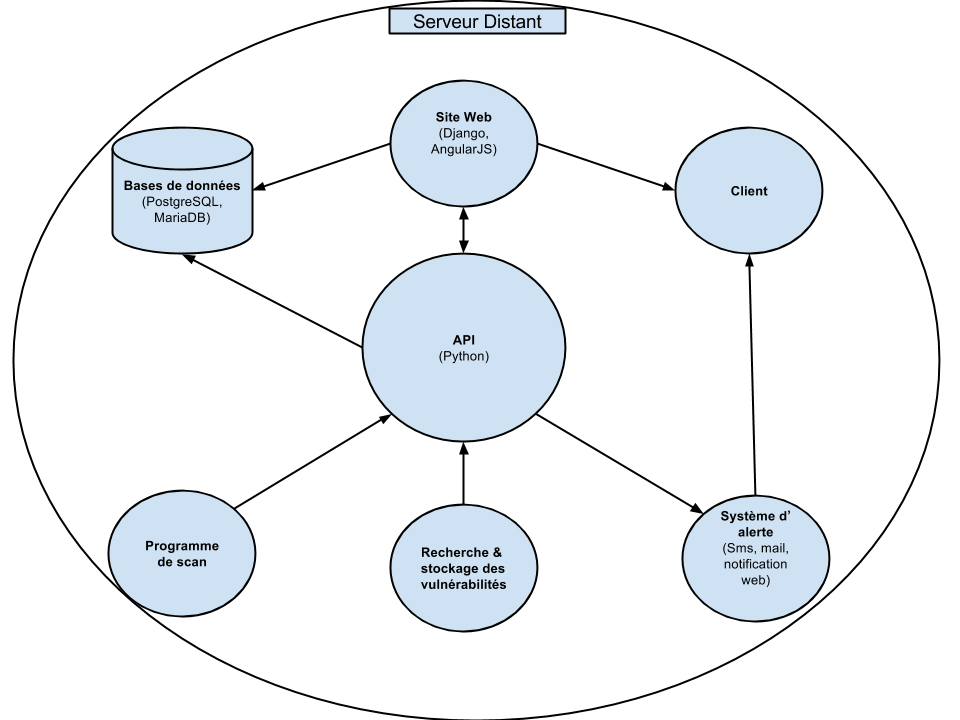
\includegraphics[width=18cm]{serveur-distant.png}
\end{figure}

\begin{figure}
  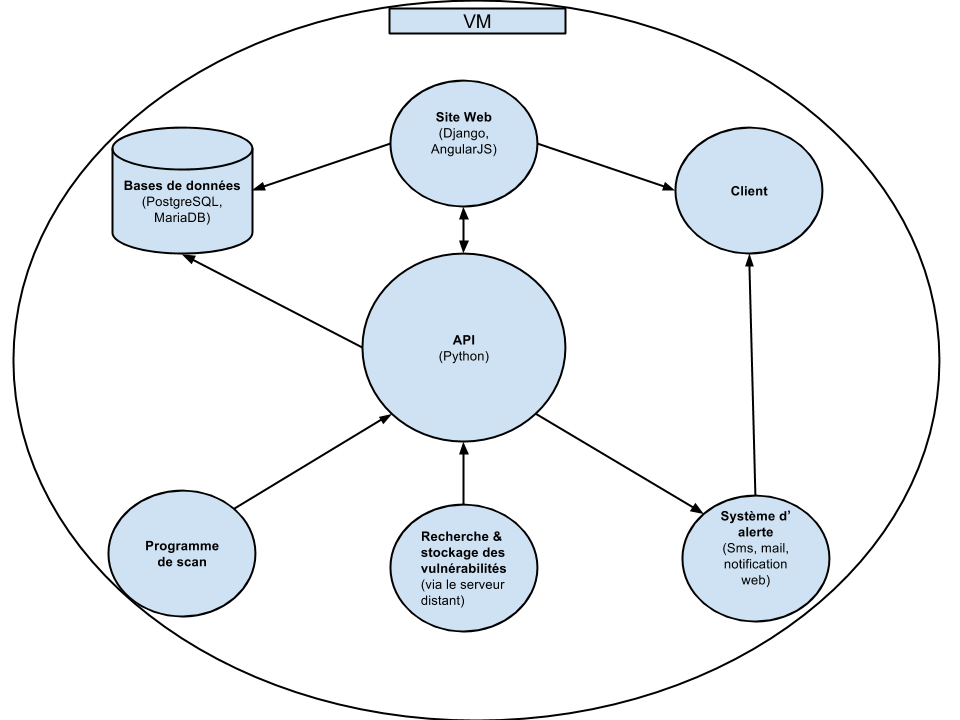
\includegraphics[width=18cm]{vm.png}
\end{figure}
\textcolor{myBlue}{\chapter{Choix des technologies}}
\section{Infrastructure}
Deux types d'infrastructures seront disponibles:
\begin{itemize}
\item Infrastructure web, hébergé sur un serveur en ligne qui nous appartient
\item Infrastructure web, hébergé sur une VM chez le client\\
\end{itemize}

Alternatives non choisies:
\begin{itemize}
\item Client lourd: pas besoin d'installation pour l'utilisateur.
\item Application mobile: pas très professionnel, moins simple d'utilisation.
\end{itemize}

\begin{figure}[!h]
  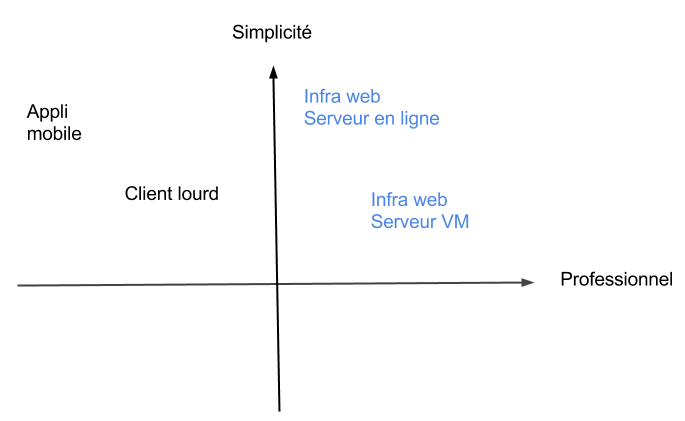
\includegraphics[width=18cm]{choix-infra.png}
\end{figure}

\newpage


\section{Composants logiciels}
Afin de choisir les différents composants logiciels du projet, nous nous sommes basés sur plusieurs critères :

Est-ce que la technologie est innovante ? Est-elle en constante évolution et nous permet-elle d'être en phase avec les autres choix du projet ?
La sécurité : est-ce que l'outil est pensé/orienté vers la sécurité, qu'elle soit de l'infrastructure ou du client ?
La rapidité de déploiement, de compréhension et d'exécution du composant : est-il facile à prendre en main, efficace ? Est-ce que la courbe d'apprentissage du composant correspond effectivement à nos besoins et à l'évolution du projet ?

\small
\begin{tabular}{| >{\raggedright}p{2.6cm}| >{\raggedright}p{3.5cm}| >{\raggedright}p{2cm}|p{7cm}|}
  \hline
  \rowcolor{Gainsboro}
  \color{Navy}{\bfseries{Choix des technologies Domaines}} & \color{Navy}{\bfseries{Technologies disponibles}} & \color{Navy}{\bfseries{Choix Vigilate}} & \color{Navy}{\bfseries{Justification}}\\
  \hline
  Framework Web & Ruby On Rails, Django, Symphony & Django & Innovant, En évolution, Orienté sécurité, En phase avec le langage de développement, Léger \\
  \hline
  Framework Javascript & jQuery, AngularJS & AngularJS & Complémentaire à Django Constante Evolution \\
  \hline
  Serveur HTTP & Apache, Nginx, Lighthttpd & Nginx & Performant, Léger \\
  \hline
  Langage de programmation & Ruby, Python, PHP & Python & Mise en place rapide, Grande flexibilité, Mutliplate-forme \\
  \hline
  Virtualisation & VmWare, VirtualBox, XEN & VirtualBox & OpenSource, Simple d’utilisation, Personnalisable \\
  \hline
  Base de données & MySQL, MariaDB, Sqlite, PostgreSQL & MariaDB, PostgreSQL & OpenSource, Simple d’utilisation, Générique\\
  \hline
\end{tabular}
\normalsize

\section{Multi OS et Multi DB}
N/A
\section{Mobile}
N/A


\end{document}